%%%%%%%%%%%% Attribution %%%%%%%%%%%%
% This template was created by 
% Chuck F. Rocca at WCSU and may be
% copied and used freely for 
% non-commercial purposes.
% 10-17-2021
%%%%%%%%%%%%%%%%%%%%%%%%%%%%%%%%%%%%%

%%%%%%% Start Document Header %%%%%%%
% In creating a new document
% copy and paste the header 
% as is.
%%%%%%%%%%%%%%%%%%%%%%%%%%%%%%%%%%%%%

\documentclass{article}

%%%% Header Information %%%%
    %%% Document Settings %%%%
    \usepackage[utf8]{inputenc}
    \usepackage[
        twoside,
        top=1in,
        bottom=0.75in,
        inner=0.5in,
        outer=0.5in
    ]{geometry}
    \pagestyle{myheadings}

%%%% Additional Commands to Load %%%%
    \usepackage{tcolorbox}
    \tcbuselibrary{skins}
    \usepackage{minted}
    \usepackage{color}
    \usepackage{tikz}
    \usetikzlibrary{calc}
    \usepackage{tabularx,colortbl}
    \usepackage{amsfonts,amsmath,amssymb}
    \usepackage{titling}
    \usepackage{mathrsfs}
    \usepackage{calc}
    \usepackage{xepersian}

%%%% Commands to Define Homework Boxes %%%%
%%%% Box Definition %%%%
    \newtcolorbox{prob}[1]{
    % Set box style
        sidebyside,
        sidebyside align=bottom,
    % Dimensions and layout
        width=\textwidth,
        toptitle=2.5pt,
        bottomtitle=2.5pt,
        righthand width=0\textwidth,
    % Coloring
        colbacktitle=gray!30,
        coltitle=black,
        colback=white,
        colframe=white,
    % Title formatting
        title={
            #1 \hfill نمره:\phantom{WWWW}
        },
        fonttitle=\large\bfseries
    }

%%%% Environment Definition %%%%
    \newenvironment{problem}[1]{
        \begin{prob}{#1}
    }
    {
        \tcblower
        \centering
        \vspace{\baselineskip}
        \end{prob}
    }



%%%% Document Information %%%%
    \title{\lr{HW2 Solutions}}
    \author{\lr{Written By Reza Shahriari}}
    \date{}

%%%%%%% End Document Header %%%%%%%


%%%% Begin Document %%%%
% note that the document starts with
% \begin{document} and ends with
% \end{document}
%%%%%%%%%%%%%%%%%%%%%%%%
\settextfont{BNAZANIN.TTF}

\begin{document}

%%%% Format Running Header %%%%%
\markboth{\theauthor}{\thetitle}

%%%% Insert the Title Information %%%
\maketitle


%%%% General Description of the Document %%%%


\raggedleft
%%%% Introduction to the General Template %%%%
\section{بخش مقدماتی (35 نمره)}
\centering
\lr{Disclaimer:} 

\lr{This is the solution manual to the homework assigned to students of Digital Control - Dr.Talebi.}

\lr{We do not guarantee that this solution is precise and thorough so please contact your TA to propose your innovative solutions and/or any probable mistakes.}


    \begin{problem}{سوال اول}
    \raggedleft
    \lr{Solution:}
    
    $\frac{X(z)}{z} = \frac{2z^2+1}{(z-2)^2(z-1)} = \frac{9}{(z-2)^2} - \frac{1}{z-2} + \frac{3}{z-1}$
    
    \lr{then}
    
    $X(z) = \frac{9z^{-1}}{(1-2z^-1)^2} - \frac{1}{1-2z^-1} + \frac{3}{1-z^-1}$
    
    \lr{At last we have} :
    
    $x(k) = 9k(2^{k-1}) - 2^k + 3$
    
    
    \end{problem}

    \begin{problem}{سوال دوم}
    \raggedleft
    \lr{Firstly : Decompose the Transfer function to the following :}
    
    $G(z)  = \frac{1}{z-0.1} \frac{z-2}{z^2 - 0.5z +1}$
    
    \lr{Realize the first part:}
    
    $G_{FP} = \frac{z^{-1}}{1-0.1z^{-1}}$
    
    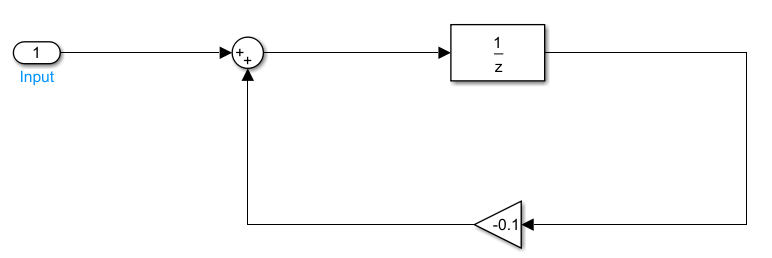
\includegraphics[width=\linewidth]{Second Series/8.png}
    
    \lr{Now Realize the second part:}
    
    $G_{ُSP} =\frac{z^{-1} - 2z^{-2}}{1 - 0.5z^{-1} +z{-2}}$
    
    \lr{Use Observable Canonical :}
    
    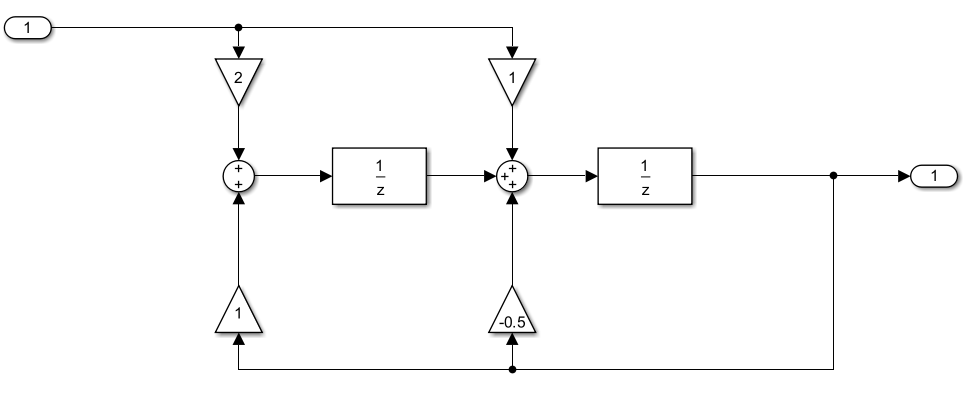
\includegraphics[width=\linewidth]{Second Series/9.png}
    
    \lr{Bring the two realized parts together to have the realized block diagram.}
    
    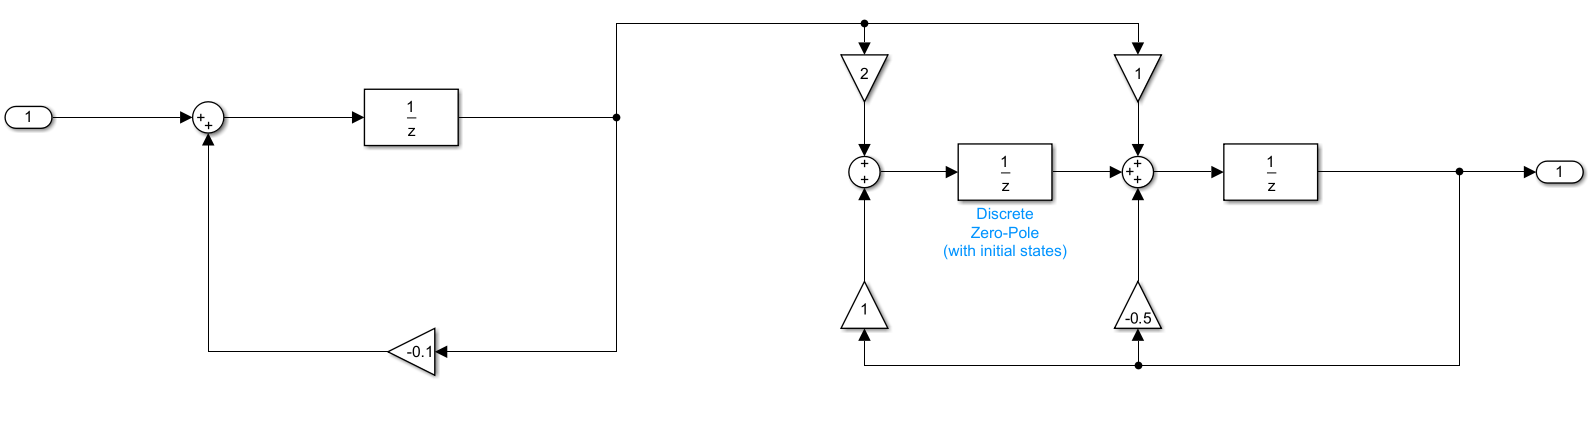
\includegraphics[width=\linewidth]{Second Series/10.png}
    \end{problem}
    
    \begin{problem}{ادامه سوال دوم}
    	\raggedleft
    	\lr{What happens if we were asked the same question but with the parallel implementation:}
    	
    	\lr{Steps are as before: (Do it yourself as an exercise)}
    	
    	$G(z) = \frac{1.979z^{-1} + 0.21z^{-2}}{1 - 0.5z^{-1} + z^{-2}} + \frac{-1.979z^{-1}}{1 - 0.1z{-1}}$
    	
    	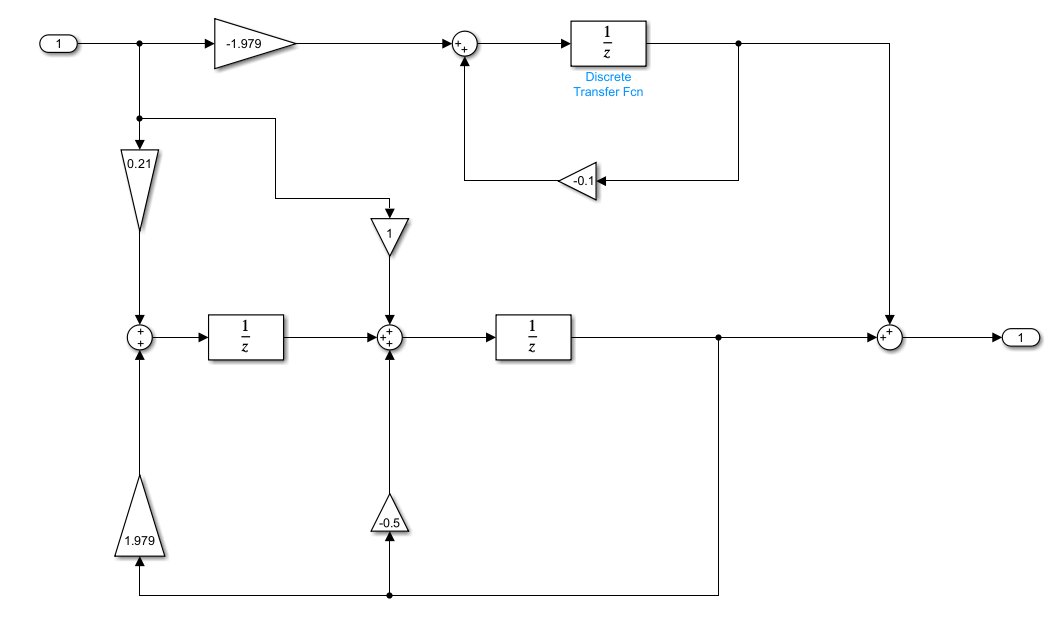
\includegraphics[width=\linewidth]{Second Series/18.png}
    \end{problem}
    
    \begin{problem}{سوال سوم}
    	\raggedleft
    	$-\frac{1}{s}U(s)e^{-sT} + \frac{1}{s}U(s) = Y(s)$
    	
    	\lr{The transfer function would be:}
    	
    	$G(s) = \frac{1-e^{-sT}}{s}$ 
    	
    	\lr{This is the ZOH transfer function.}
    	
    \end{problem}
    \begin{figure}[htbp]
    	\centering
    	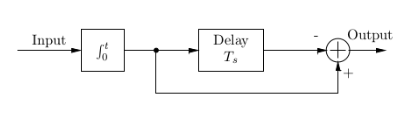
\includegraphics{Second Series/4.png}
    	\caption{شکل سوال سوم}
    \end{figure}
    
    
    \begin{problem}{سوال چهارم}
    	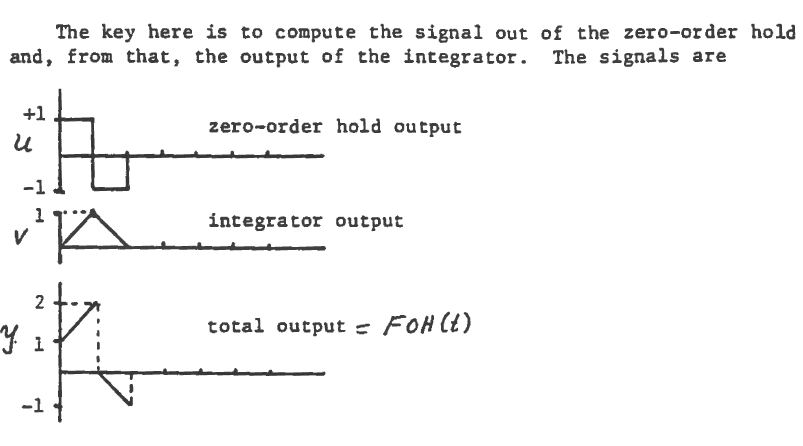
\includegraphics[width=\linewidth]{Second Series/17.png}
    	
    	
    \end{problem}
    \begin{figure}[htbp]
    	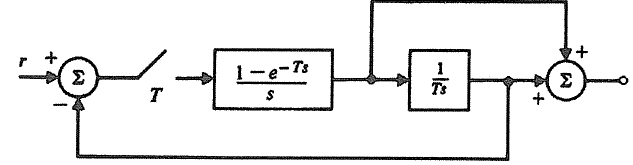
\includegraphics[width=\linewidth]{Second Series/5.png}
    	\caption{شکل سوال چهارم}
    \end{figure}
    
    \begin{problem}{سوال پنجم}
    	\lr{Based on what we have seen in Section 3.4 of Digital control systems by C.L.Phillips (2015) we have:}
    	
    		\begin{equation}
    			{{E}^{*}}(s)=\sum\limits_{\begin{smallmatrix} 
    					at\,poles\, \\ 
    					of\,E(\lambda ) 
    			\end{smallmatrix}}{[residues\,of\,E(\lambda )}\frac{1}{1-{{\varepsilon }^{-T(s-\lambda )}}}]
    		\end{equation}
    		
    		\raggedleft
    		\lr{The Starred transform would be as noted bellow:}
    		\centering
    		
    		$\frac{2}{1-e^{-Ts}} + \frac{-1}{1-e^{T(s+1)}}$
    	
    \end{problem}
\raggedleft    
\section{بخش متوسط (35 نمره)}
\centering
حل \underline{دو سوال} از این بخش الزامی است.
\begin{problem}{سوال ششم}
	\raggedleft
	\lr{For the first part you can substitute k in the given range to calculate what is asked.}
	
	\lr{Second Part:}
	
	\lr{recall that we had :}
	
	$y(k+2) = Z^2Y(z) - Zy(1) - y(0)$
	
	\lr{now take z transform from the difference equation:}
	
	$Z^2Y(z) - \frac{3}{4}ZY(z) + \frac{1}{8}Y(z) = E(z) $
	
	$(Z^2 - \frac{3}{4}Z + \frac{1}{8}) Y(z) = E(z)$
	
	$\frac{Y(z)}{E(z)} = \frac{1}{Z^2 - \frac{3}{4}Z + \frac{1}{8}}$
	
	\lr{The transfer function is unstable.}
	
	

\end{problem}
	

\begin{problem}{سوال هفتم}
	\raggedleft
	\lr{Based on the block diagram we have:}
	
	$y(k) = \beta_2 e(k) + \beta_1 e(k-1) + \beta_0 e(k-2) - \alpha_1 y(k-1) - \alpha_0 y(k-2)$
	
	\lr{Take z transform:}
	
	$(1 + \alpha_1 Z^{-1} + \alpha_0 Z^{-2}) Y(z) = (\beta_2 + \beta_1 Z^{-1} \beta_0 Z^{-2})E(z)$
	
	\lr{Find the transfer function:}
	
	$\frac{Y(z)}{E(z)} = \frac{(\beta_2 + \beta_1 Z^{-1}+ \beta_0 Z^{-2})}{(1 + \alpha_1 Z^{-1} + \alpha_0 Z^{-2})} $
	
	\lr{Which would be equal to :}
	
	$\frac{Y(z)}{E(z)} = \frac{(\beta_2Z^2 + \beta_1 Z+ \beta_0)}{(Z^2 + \alpha_1 Z + \alpha_0)} $
	
	\lr{So we would have:}
	
	$\beta_2 = 2, \beta_1 = -2.4, \beta_0 = 0.72 $
	
	$\alpha_1 = -1.4, \alpha_0 = 0.98 $
	
\end{problem}
\begin{figure}
	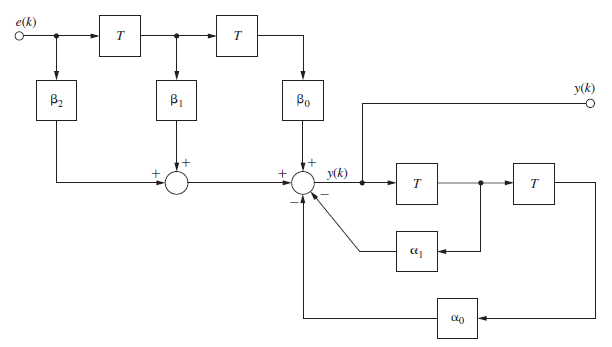
\includegraphics[width=\linewidth]{Second Series/2.png}
	\caption{شکل سوال هفتم}
\end{figure}

\begin{problem}{سوال هشتم}
	\raggedleft
	\lr{The block diagram represents the following difference equation:}
	
	$f(k) = -\alpha_1f(k-1) -\alpha_0f(k-2) + e(k)$
	
	$y(k) = b_2f(k) + b_1f(k-1) + b_0f(k-2)$
	
	\lr{Now take the z-transform:}
	
	$F(z) = (-\alpha_1Z^{-1} + -\alpha_0Z^{-2})F(z) + E(z)$
	
	$Y(z) = (b_2 + b_1Z^{-1} + b_0Z^{-2})F(z)$
	
	\lr{Now derive the transfer function:}
	
	$\frac{F(z)}{E(z)} = \frac{1}{1 + \alpha_1Z^{-1} + \alpha_0Z^{-2}}$
	
	$\frac{Y(z)}{F(z)} = (b_2 + b_1Z^{-1} + b_0Z^{-2})$
	
	$\frac{Y(z)}{E(z)} = \frac{b_2 + b_1Z^{-1} + b_0Z^{-2}}{1 + \alpha_1Z^{-1} + \alpha_0Z^{-2}}$
	
	\lr{Which is equivalent to :}
	
	$\frac{Y(z)}{E(z)} = \frac{b_2Z^2 + b_1Z + b_0}{Z^2 + \alpha_1Z + \alpha_0}$
	
	$b_2 = 2, b_1 = -2.4, b_0 = 0.72 $
	
	$\alpha_1 = -1.4, \alpha_0 = 0.98 $
	




\end{problem}
\begin{figure}
	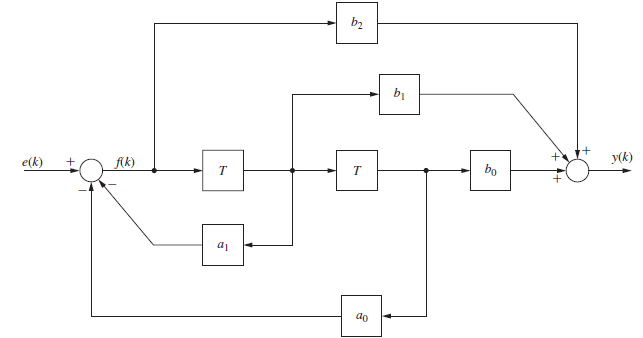
\includegraphics[width=\linewidth]{Second Series/3.png}
	\caption{شکل سوال هشتم}
\end{figure}


\begin{problem}{سوال نهم}
	\raggedleft
	\lr{Recall the following equation:}
	
	$G(z)=(1-{{z}^{-1}})\,{{Z}}\{\frac{G(s)}{s}\}$
	
	\lr{using the equation we have the following ZOH-equavalent transfer function:}
	
	$\frac{1}{2} + \frac{-e(1-Z^{-1})}{1- e^{-T}Z^{-1}} + \frac{\frac{1}{2} e^2(1-Z^{-1})}{1-e^{-2T}Z^{-1}}$
	
	\lr{Where T must be substituted to 0.5}
	

	
\end{problem}
\begin{problem}{سوال دهم}
	\raggedleft
	\lr{recall that :}
	
	\centering
	\begin{equation}
		\cos \omega n\overset{*}{\longleftrightarrow}[\frac{{{e}^{sT}}({{e}^{sT}}-\cos \omega )}{{{e}^{2sT}}-2{{e}^{sT}}\cos \omega +1}]
	\end{equation}
	
	\raggedleft
	\lr{now calculate it for the two given functions}
	
	$1) [\frac{{{e}^{sT}}({{e}^{sT}}-\cos 4\pi T )}{{{e}^{2sT}}-2{{e}^{sT}}\cos 4\pi T +1}] $
	
	$2) [\frac{{{e}^{sT}}({{e}^{sT}}-\cos 16\pi T )}{{{e}^{2sT}}-2{{e}^{sT}}\cos 16\pi T +1}]$
	
	\lr{It is now evident why the starred transform are the same.}
	
	\raggedleft
	
	
\end{problem}

\raggedleft
\section{ بخش تکمیلی (30 نمره)}
\centering
حل \underline{دو سوال} از این بخش الزامی است.
\begin{problem}{سوال یازدهم}
	\raggedleft
	\lr{The main idea of solving this kind of questions is paying attention to the stability and Final Value Theorem.}
	
	\lr{Note that the given figures are the step response of the transfer functions. Meaning that you take into account a $\frac{1}{1-Z^{-1}}$ term multiplied by the transfer function.}
	
	\lr{Based on what is said we now begin to identify the unstable outputs.}
	
	\lr{$\bullet$ $G_4$ is unstable with having repeated poles on z = 1. This is C.}
	
	\lr{$\bullet$ $G_6$ is unstable for having a poles on z = 1.2. This is E.}
	
	\lr{The rest are stable.}
	
	\lr{$\bullet$Poles of $G_1$ are -0.1 and -0.7. We know that negative poles cause the step response to be oscillatory so both A and B could be the answer. In order to determine which the answer is, we use final value theorem which equals to 0.534759 this closer to B.}
	
	\lr{$\bullet$Poles of $G_2$ are 0.1 and 0.7. Both F and D could be the answer. In order to determine exactly which the answer is, we use final value theorem which equals to 3.70 this closer to D.}
	
	\lr{$\bullet$Poles of $G_3$ are 0.1 and 0.1. Both F and D could be the answer. In order to determine exactly which the answer is, we use final value theorem which equals to 1.23 this closer to F.}
	
	\lr{$\bullet$Poles of $G_5$ are 0.4 - 0.6i and 0.4 + 0.6i. It is in the stable region. In order to determine exactly which the answer is, we use final value theorem which equals to 1.38 this is A.}
	
	
	
\end{problem}
\begin{figure}[htbp]
	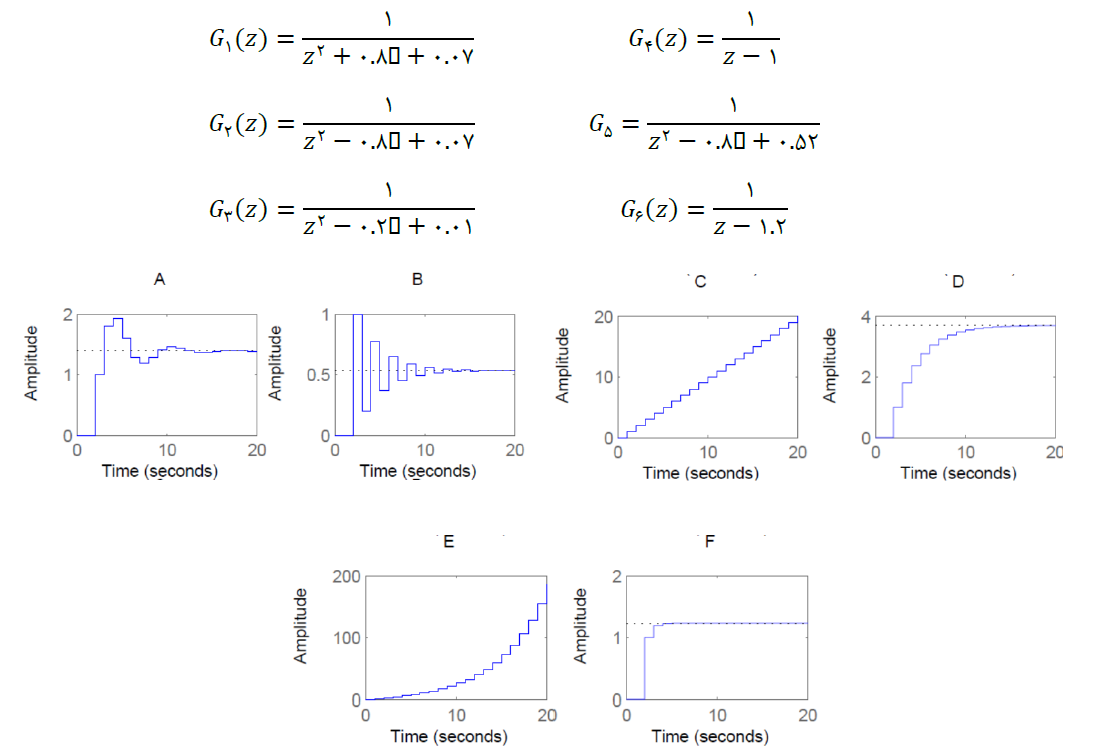
\includegraphics[width=\linewidth]{Second Series/1.png}
	\caption{شکل سوال یازدهم}
\end{figure}


\begin{problem}{سوال دوازدهم}
	\raggedleft
	\lr{As you can see in the picture below we could write:}
	
	* $C(s) = G_1(s) f(s)$
	
	$f(s) = R(s) -D^*(s)C^*(s) - G_2(s)C(s)$
	
	** $C(s) = \frac{R(s)G_1(s)}{1+G_1(s)G_2(s)} - \frac{G_1D^*(s)C^*(s)}{1+G_1(s)G_2(s)}$
	
	$C^*(s) = (\frac{R(s)G_1(s)}{1+G_1(s)G_2(s)})^* - (\frac{G_1}{1+G_2})^* D^*(s)C^*(s) $
	
	$C^*(s)(1 + (\frac{G_1}{1+G_2})^* D^*(s)) = (\frac{R(s)G_1(s)}{1+G_1(s)G_2(s)})^*$
	
	$C^*(s) = \frac{(\frac{R(s)G_1(s)}{1+G_1(s)G_2(s)})^*}{(1 + (\frac{G_1}{1+G_2})^* D^*(s))}$
	
	\lr{Now use the equation derived above inside the $**$ equation and then use it in the * equation to get the following:}
	
	$C(s) = \frac{R(s)G_1(s)}{1+G_1(s)G_2(s)} - \frac{G_1D^*(s)(\frac{(\frac{R(s)G_1(s)}{1+G_1(s)G_2(s)})^*}{(1 + (\frac{G_1}{1+G_2})^* D^*(s))})}{1+G_1(s)G_2(s)} $
	
	\lr{Similarly:}
	
	$C(z) = \frac{R(z)G_1(z)}{1+G_1(z)G_2(z)} - \frac{G_1D^*(z)(\frac{(\frac{R(z)G_1(z)}{1+G_1(z)G_2(z)})^*}{(1 + (\frac{G_1}{1+G_2})^* D^*(z))})}{1+G_1(z)G_2(z)} $
	
	
\end{problem}
\begin{figure}
	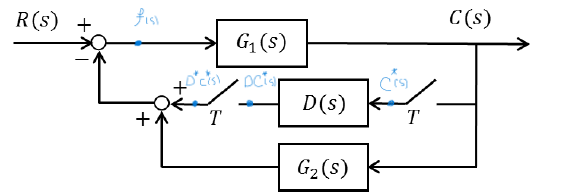
\includegraphics[width=\linewidth]{Second Series/6.png}
	\caption{شکل سوال دوازدهم}
\end{figure}
\begin{problem}{سوال سیزدهم}
	\raggedleft
	\lr{As you can see in the picture below we could write:}
	
	$E(s) =R(s) - H(s)Y(s)$
	
	$Y(s) = G_2(s)E(s) + G_1(s)E^*(s)$
	
	\lr{Draw the original SFG:}
	
	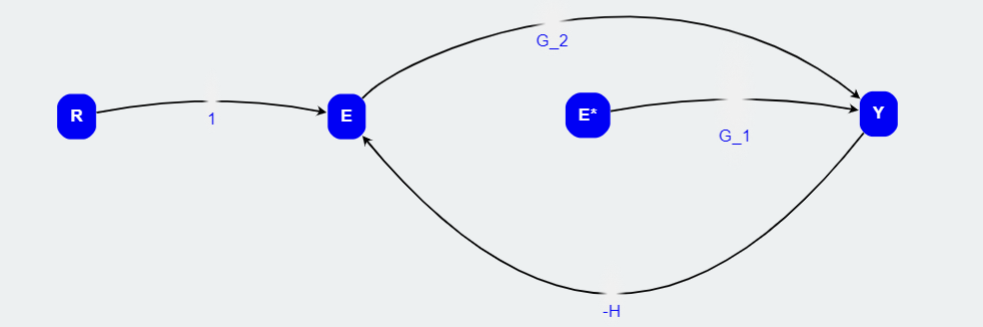
\includegraphics[width=\linewidth,]{Second Series/12.png}
	
	\lr{Change the equations so that Y is written in terms of R:}
	
	$Y(s) = G_2(s)(R(s) - H(s)Y(s)) + G_1(s)E^*(s)$
	
	$Y(s) +  G_2(s)H(s)Y(s) = G_2(s)R(s) + G_1(s)E^*(s)$
	
	$(1 + G_2(s)H(s))Y(s) = G_2(s)R(s) + G_1(s)E^*(s)$
	
	$Y(s) = \frac{G_2(s)R(s)}{(1 + G_2(s)H(s))} + \frac{G_1(s)E^*(s)}{(1 + G_2(s)H(s))}$
	
	$E(s) = \frac{R(s)}{1 + G_2(s)H(s)} - \frac{G_1(s)H(s)}{1 + G_2(s)H(s)} E^*(s)$
	
	$E^*(s) = (\frac{R(s)}{1 + G_2(s)H(s)})^* - (\frac{G_1(s)H(s)}{1 + G_2(s)H(s)})^* E^*(s)$
	
	\lr{Compute the starred transform:}
	
	$Y^*(s) = (\frac{G_2(s)R(s)}{(1 + G_2(s)H(s))})^* + (\frac{G_1(s)}{(1 + G_2(s)H(s))})^* E^*(s)$
	
	\lr{Three equations that help us draw the modified SFG:}
	
	
	$Y(s) = \frac{G_2(s)R(s)}{(1 + G_2(s)H(s))} + \frac{G_1(s)E^*(s)}{(1 + G_2(s)H(s))}$
	
	
	$Y^*(s) = (\frac{G_2(s)R(s)}{(1 + G_2(s)H(s))})^* + (\frac{G_1(s)}{(1 + G_2(s)H(s))})^* E^*(s)$
	
	$E^*(s) = (\frac{R(s)}{1 + G_2(s)H(s)})^* - (\frac{G_1(s)H(s)}{1 + G_2(s)H(s)})^* E^*(s)$
	
	
	\lr{Let's write it in a more summarized manner:}
	
	$Y(s) = G_3 R(s) + G_4 E^*(s)$
	
	$Y^*(s) = (G_3 R(s))^* +  G_4^* E^*(s) $
	
	$E^* = G_6 + G_5 E^*(s)$
	
	\lr{It is obvious that we have:}
	
	$G_3 = (\frac{G_2(s)}{(1 + G_2(s)H(s))}) $
	
	$G_4 = (\frac{G_1(s)}{(1 + G_2(s)H(s))})$
	
	$G_5 = (\frac{G_1(s)H(s)}{1 + G_2(s)H(s)})^*$
	
	$G_6 = (\frac{R(s)}{1 + G_2(s)H(s)})^* $ 
	
	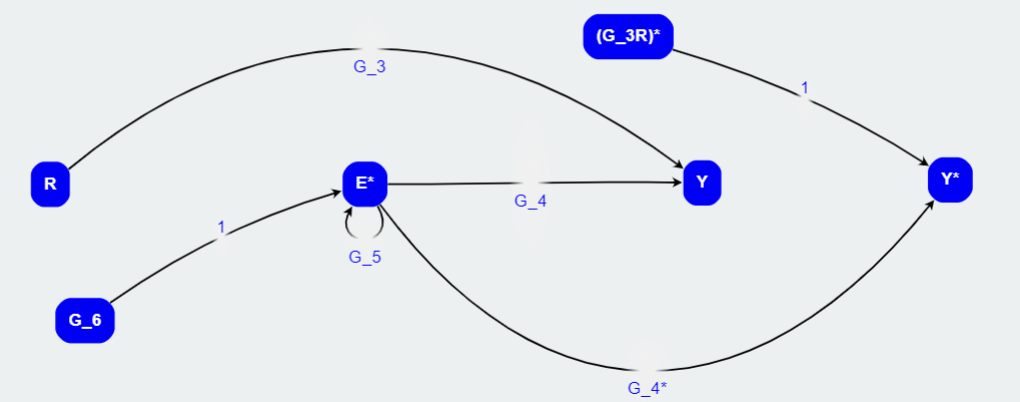
\includegraphics[scale=0.7]{Second Series/13.png}
	
\end{problem}

\begin{problem}{ادامه سوال سیزدهم}
	\raggedleft
	\lr{In the previous page, you can see the modified SFG.}
	
	\lr{Obviously, you could derive $\frac{Y(s(z))}{R(s(z))}$ but not the $\frac{Y(s)}{R^*(s)}$}
\end{problem}

\begin{figure}
	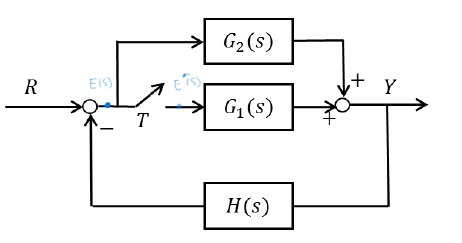
\includegraphics[width=\linewidth]{Second Series/7.png}
	\caption{شکل سوال سیزدهم}
\end{figure}

\begin{problem}{سوال چهاردهم}
	\raggedleft
	\lr{Just like what we had in the second question, but here it is parallel, whereas in the Second question the Series implementation is asked:}
	
    $G(z) = \frac{-2.1575}{(z-0.1)} + \frac{2.1875z-1.875}{(z^2-0.5z+1)}$
    
    \lr{implement the first transfer function:}
    
    $G_1(z) = \frac{-2.1575z^{-1}}{1 - 0.1z^{-1}}$
    
    $G_2(z) = \frac{2.1875z^{-1}+ 1.875z^{-2}}{(1-0.5z^{-1}+z^{-2})}$
    
    \lr{we implement $G_1$:}
    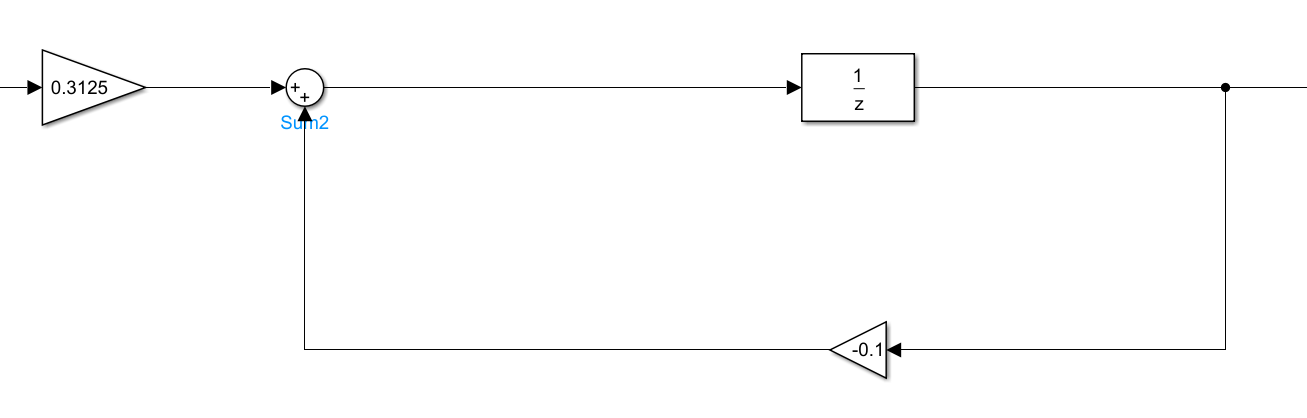
\includegraphics[width=\linewidth]{Second Series/14.png}
    
    \lr{we implement $G_2$:}
    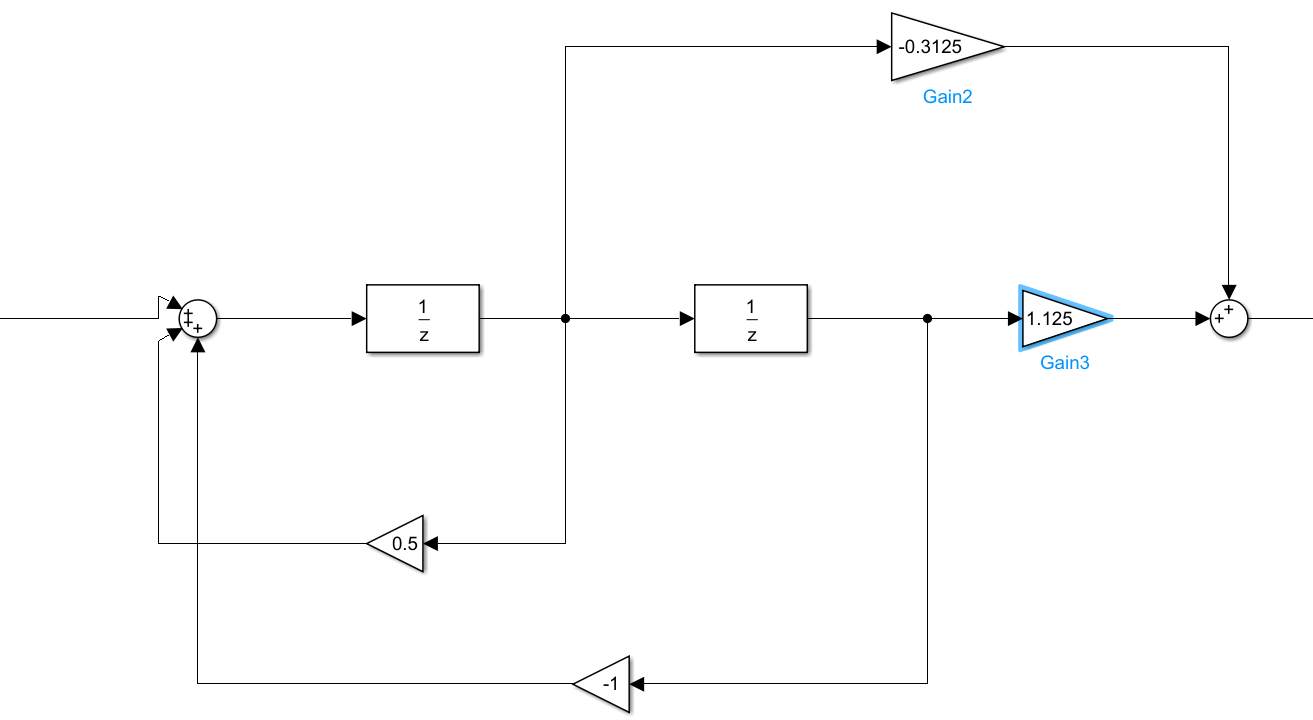
\includegraphics[width=\linewidth]{Second Series/15.png}
    
    
	
\end{problem}

\begin{problem}{ادامه سوال چهاردهم}
	\raggedleft
	\lr{Now put them together}
	
	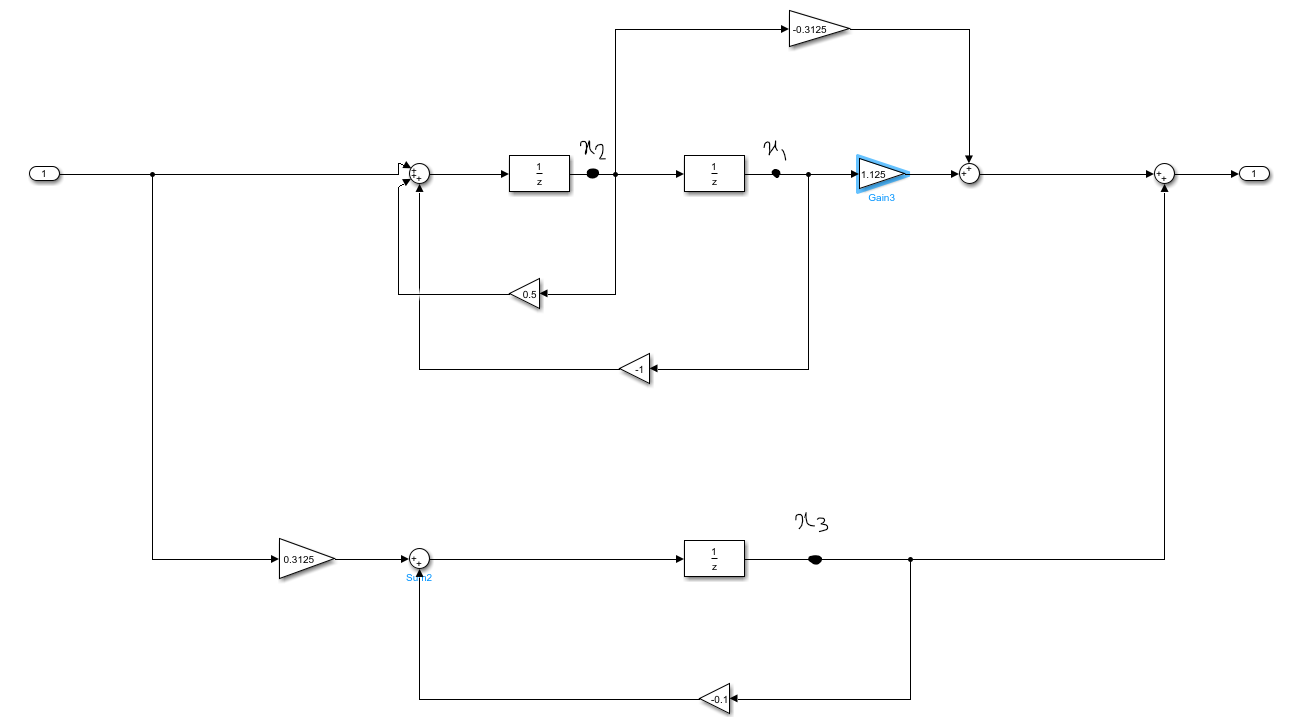
\includegraphics[width = \linewidth]{Second Series/16.png}
	
	\lr{Now for the second part of the problem}
	
	 \begin{align}
		& \left( \begin{matrix}
			{{{\dot{x}}}_{1}}  \\
			{{{\dot{x}}}_{2}}  \\
			{{{\dot{x}}}_{3}}  \\
		\end{matrix} \right)=\left( \begin{matrix}
			0 & 1 & 0  \\
			0.5 & -1 & 0  \\
			0 & 0 & -0.1  \\
		\end{matrix} \right)\left( \begin{matrix}
			{{x}_{1}}  \\
			{{x}_{2}}  \\
			{{x}_{3}}  \\
		\end{matrix} \right)+\left( \begin{matrix}
			0  \\
			1  \\
			0.3125  \\
		\end{matrix} \right)u \\ 
		& y=\left( \begin{matrix}
			1.125 & \begin{matrix}
				-0.3125 & 1  \\
			\end{matrix}  \\
		\end{matrix} \right)\left( \begin{matrix}
			{{x}_{1}}  \\
			{{x}_{2}}  \\
			{{x}_{3}}  \\
		\end{matrix} \right) \\ 
	\end{align}
	

	
	
\end{problem}


\begin{problem}{سوال پانزدهم}
	\raggedleft
	\lr{Use the following equation again:}
	
	$G(z)=(1-{{z}^{-1}})\,{{Z}}\{\frac{G(s)}{s}\}$
	
	\lr{We get:}
	
	$\frac{b}{a} + \frac{a-b}{a} \frac{1-z^{-1}}{1-e^{-aT}z^{-1}}$
	
	\lr{which is equal to :}
	
	$\frac{1 - (\frac{b}{a}e^{-aT} + \frac{a-b}{a})z^{-1}}{1 - e^{-aT}z^{-1}}$
	
	\lr{Which is always non-minimum phase here is why:}
	
	\lr{The zero is $(\frac{b}{a}e^{-aT} + \frac{a-b}{a})$ let us rewrite it like bellow:}
	
	$\frac{b}{a}(e^{-aT} - 1) + 1$
	
	\lr{Since $\frac{b}{a}$ is always negative and similarly $(e^{-aT} - 1)$ is always negative, the first term is always positive. Which means the zero is always greater than 1, hence the system is non-minimum phase.}
	
	
	
	
\end{problem}


\end{document}
